%
% ==============================================================================
\section{Event-based PSHA calculator}
\label{chap:stochastic_psha}
%
The calculation of a \gls{stochasticeventset} \index{Stochastic event set} 
and the corresponding \glspl{groundmotionfield} is procedure particularly 
suited for seismic risk calculations involving a number of assets located 
at close distance to each other.
%
OpenQuake, given a \gls{seismicsourcesystem}, can generate a number of 
\glspl{seismicityhistory}, each one representing a possible realisation of 
the seismicity originated by a \gls{seismicsourcemodel} during a given 
investigation time (fixed by the user). 
%
The ensamble of these \glspl{seismicityhistory} is called a 
\gls{acr:ses} .

Each rupture in a seismicity history is successively associated with a ground
motion field, an object describing the spatial distribution of a scalar 
parameter representative of the intensity of shaking (e.g. PGA or Spectral 
Acceleration). 
%
% ------------------------------------------------------------------------------
\subsection{Stochastic Event Set Calculator}
\index{Seismicity History}
\index{Stochastic event set}
A stochastic event set (SES) is collection of seismicity histories; a 
seismicity history contains earthquake ruptures obtained by randomly 
sampling an \gls{earthquakeruptureforecast}. 
%
As described in Chapter \ref{chap:erf}, an \gls{acr:erf} is defined 
as the inventory of all ruptures produced by a \gls{seismicsourcemodel}, 
together with their probabilities of occurrence over a specified time span.

Currently OpenQuake supports the capability to generate SESs from 
Poissonian \glspl{acr:erf}. In a Poissonian ERF, the probability of one
or more occurrences in a time span $t$ associated to each rupture is 
given by:
%
\begin{equation}
P(\#rup\geq1|t) = 1 - \exp(-\nu t)
\end{equation} 
where $\nu$ is annual rate of occurrence of the rupture. Knowing 
$P(\#rup\geq1|t)$, it is possible to derive the expected number of 
earthquake ruptures ($\lambda$) in the time span $T$  as:
\begin{equation}
\lambda = - \ln(1 - P_{i}(\#rup\geq1|t))
\end{equation} 
The Poisson probability of having $\#rup$ ruptures given $\lambda$ 
expected ruptures can be then computed as:
%
\begin{equation}
P(\#rup;\lambda) = \exp(-\lambda)\frac{\lambda^{n}}{n!}
\label{ses:p}
\end{equation}
\marginpar{this equation \ref{ses:p} is not clear}
%
For each rupture, the number of occurrences in a time span $T$ 
can be then obtained as a random sample of the Poisson probability 
density function described in equation \ref{ses:p}. By looping over
all the ruptures in a ERF, it is therefore possible to simulate a 
stochastic event set where each rupture is present (zero, one or 
more times) according to the input probability. 
%
In other words, the resulting collection of sampled ruptures represents 
a possible realization of the seismicity as described by the ERF. 
%
By sampling an \gls{acr:erf} multiple times, different \glspl{acr:ses} 
can be obtained each representing a possible realization of the seismic 
activity. 
As an example, Figure \ref{ses_italy} shows two SESs produced by a 
fault model for the Italian region (derived from the Italian fault 
database \citep{basili2008}). 
%
Each SES represents seismicity for a period of 50 years. The two 
\glspl{acr:ses} shows similar spatial distribution of seismicity (as 
expected given that they come from the same source model), but the 
location and magnitude of the events is different due to the fact that 
they depict two different 'possible' realizations of seismic activity 
in the region.
% ..............................................................................
% . . . . . . . . . . . . . . . . . . . . . . . . . . . . . . . . . . . > Figure
\begin{figure}[!htbp]
\begin{center}
\subfigure[]{
\includegraphics[width=12cm]{./Figures/Part_Hazard/DissEventSet1.eps}}
\subfigure[]{
\includegraphics[width=12cm]{./Figures/Part_Hazard/DissEventSet2.eps}}
\caption{Different stochastic event sets (a) and (b) generated from a 
fault model for the Italian region (derived from DISS database 
\citep{basili2008}) for a period of 50 years.}
\label{ses_italy}
\end{center}
\end{figure}
% ..............................................................................
% . . . . . . . . . . . . . . . . . . . . . . . . . . . . . . . . . . . < Figure
%
% ------------------------------------------------------------------------------
\subsection{Ground Motion Field calculator}
\index{Ground Motion!Field}
The \gls{groundmotionfieldcalc} computes values of a scalar
ground motion intensity parameter (e.g. \gls{acr:pga}, \gls{acr:sa}, 
\gls{acr:pgv} as predicted 
by a GMPE) over a set of geographical locations, by utilizing a 
rupture model (described in terms of geometry and magnitude) as 
the source of shaking.

In general, a ground motion model that predicts intensities at 
an individual site $i$ due to an earthquake $j$ takes the following 
form (\cite{jayaram2009}):
%
\begin{equation}
\ln (Y_{ij}) = \ln (\overline{Y}_{ij})+\epsilon_{ij}+\eta_{j}
\label{gmfeq}
\end{equation}
%
where $Y_{ij}$ denotes the ground motion parameter of interest; 
$\overline{Y}_{ij}$ denotes the predicted median ground motion 
intensity (which depends on parameters like magnitude, distance, 
period, etc.); $\epsilon_{ij}$ denotes the intra-event residuals 
(which is a gaussian random variable with zero mean and standard 
deviation $\sigma_{ij}$); and $\eta_{j}$ denotes the inter-event 
residual, which is a gaussian random variable with zero mean and 
standard deviation $\tau_{j}$. The standard deviations $\sigma_{ij}$ 
and $\tau_{j}$ are estimated as part of the GMPE and are function of 
the spectral period of interest. The intra-event standard deviation 
may depends also on the earthquake magnitude and distance of the 
site from the rupture. During an earthquake, the inter-event residual
computed at any particular period is constant across all the sites.

For a given earthquake and a set of $N$ sites, equation \ref{gmfeq} 
can be rewritten in a vectorial form as:
\begin{equation}
\ln (\bm{Y}) = \ln (\overline{\bm{Y}})+\bm{\epsilon}+\bm{\eta} 
\label{gmfeqvec}
\end{equation}
where 
\[
{\ln (\bm{Y})}=[\ln (Y_{1}), \ln (Y_{2}),...,\ln (Y_{N})]
\]
\[
\ln (\overline{\bm{Y}})=[\ln (\overline{Y_{1}}), 
\ln (\overline{Y_{2}}),...,\ln (\overline{Y_{N}})]
\]
\[
\bm{\epsilon}=[\epsilon_{1},\epsilon_{2},...,\epsilon_{N}]
\]
and $\bm{\eta}=[\eta_{1},\eta_{2},...,\eta_{N}]$, 
where $\eta_{1}=\eta_{2}=...=\eta_{N}=\eta$.\\
Given a GMPE, the Ground Motion Field calculator can compute different types 
of ground motion fields:
\begin{itemize}
\item Median
\item Intra-Event Uncorrelated
\item Intra-Event Correlated
\end{itemize}
The median ground motion field provides for each location the median value of 
the ground shaking parameter as predicted by the GMPE. Following the notation 
of equation \ref{gmfeqvec}, the median ground motion is computed simply from 
the equation:
\begin{equation}
\ln (\bm{Y}) = \ln (\overline{\bm{Y}})
\end{equation}
The intra-event uncorrelated ground motion field calculator provides for each 
location a value of the ground shaking parameter that takes into account 
the aleatory uncertainties defined in the GMPE. In particular, for a single 
field calculation, it randomly samples the inter-event standard deviation, 
and for each location, it randomly samples the intra-event standard deviation.
%
Both the inter- and intra-event residuals are then added to the mean value of 
the ground shaking parameter. In other words, the intra-event uncorrelated 
ground motion field is computed using equation \ref{gmfeqvec} where the 
intra-event residuals are sampled from a multivariate normal distribution
with mean zero and a diagonal covariance matrix ($\bm{\Sigma}$):
\begin{equation}
\bm{\Sigma}=
\begin{bmatrix}
\sigma^{2}_{1} &  0  & \ldots & 0\\
0  &  \sigma^{2}_{2} & \ldots & 0\\
\vdots & \vdots & \ddots & \vdots\\
0  &   0       &\ldots & \sigma^{2}_{N}
\end{bmatrix}
\end{equation}
where $\sigma_{1}, \sigma_{2},...,\sigma_{N}$ are the intra-event standard 
deviations for sites $1$ to $N$.

The Intra-Event Correlated ground motion field calculator follows the same 
workflow of the uncorrelated field calculator, with the only difference that 
the intra-event residuals are assumed to be spatially correlated. 
%
In this case the intra-event residuals are sampled from a multivariate 
normal distribution with mean zero and a non-diagonal covariance matrix:
\begin{equation}
\bm{\Sigma}=
\begin{bmatrix}
\sigma^{2}_{1} &  \sigma_{1}\sigma_{2}\rho_{12}  & \ldots &  \sigma_{1}\sigma_{N}\rho_{1N}\\
\sigma_{2}\sigma_{1}\rho_{21}  &  \sigma^{2}_{2} & \ldots &  \sigma_{2}\sigma_{N}\rho_{2N}\\
\vdots & \vdots & \ddots & \vdots\\
\sigma_{N}\sigma_{1}\rho_{N1}  &   \sigma_{N}\sigma_{2}\rho_{N2}       &\ldots & \sigma^{2}_{N}
\end{bmatrix}
\end{equation}
where $\rho_{ij}$ is the correlation between intra-event residuals at site 
$i$ and $j$.

Currently, the intra-event correlated ground motion field calculator adopts 
the correlation model of \citet{jayaram2009}, according to which the 
correlation between intra-event residuals is given by:
 \begin{equation}
 \rho_{ij} = \rho(h) = \exp(-3h/b)
 \end{equation}
 where $h$ is the distance between sites $i$ and $j$. $b$ is a coefficient 
 dependent on period and site conditions at the site of interest. Two cases 
 are identified:
 \begin{itemize}
 \item case $1$: \gls{acr:vs30} values do not show or are not expected to show 
 clustering.
 \item case $2$: \gls{acr:vs30} values show or are expected to show 
 clustering.
 \end{itemize}
At short periods ($T<1$), for case $1$:
\begin{equation}
b = 8.5 + 17.2T
\end{equation}
At short periods ($T<1$), for case $2$:
\begin{equation}
b = 40.7 - 15.0T
\end{equation}
At long periods ($T\geq1$, for both cases $1$ and $2$):
\begin{equation}
b = 22.0 + 3.7T
\end{equation}
Summarizing, if \gls{acr:vs30} values do not show clustering, the 
correlation length between intra-event residuals is expected to 
increase with increasing period (with a rate that changes from 
$T<1$ to $T\geq1$). 
%
In case \gls{acr:vs30} values show clustering, for  $0\leq T<1$, the 
correlation length decreases with increasing period.

Figure \ref{fig:gmfs} depicts the different types of ground motion 
fields described. The median ground motion field is shown in Figure 
\ref{fig:gmfs} (a). 
%
In this case the aleatory uncertainties are not taken into account, 
and the ground motion pattern follows exactly the rupture geometry. 
The highest values are observed on the surface projection of the rupture, and 
decreasing values are found at increasing distances from the rupture. 
%
Figure \ref{fig:gmfs} (b) shows an intra-event uncorrelated ground motion 
field. The aleatory uncertainties are taken into account and therefore the
ground motion pattern shows a significant level of heterogeneity. 
%
When introducing the intra-event correlation [Figure \ref{fig:gmfs} (c)], 
the heterogeneity is diminished and an additional filtering is introduced 
when considering a longer period [Figure \ref{fig:gmfs} (d)].
%
\begin{figure}[htbp]
\centering
\subfigure[]{
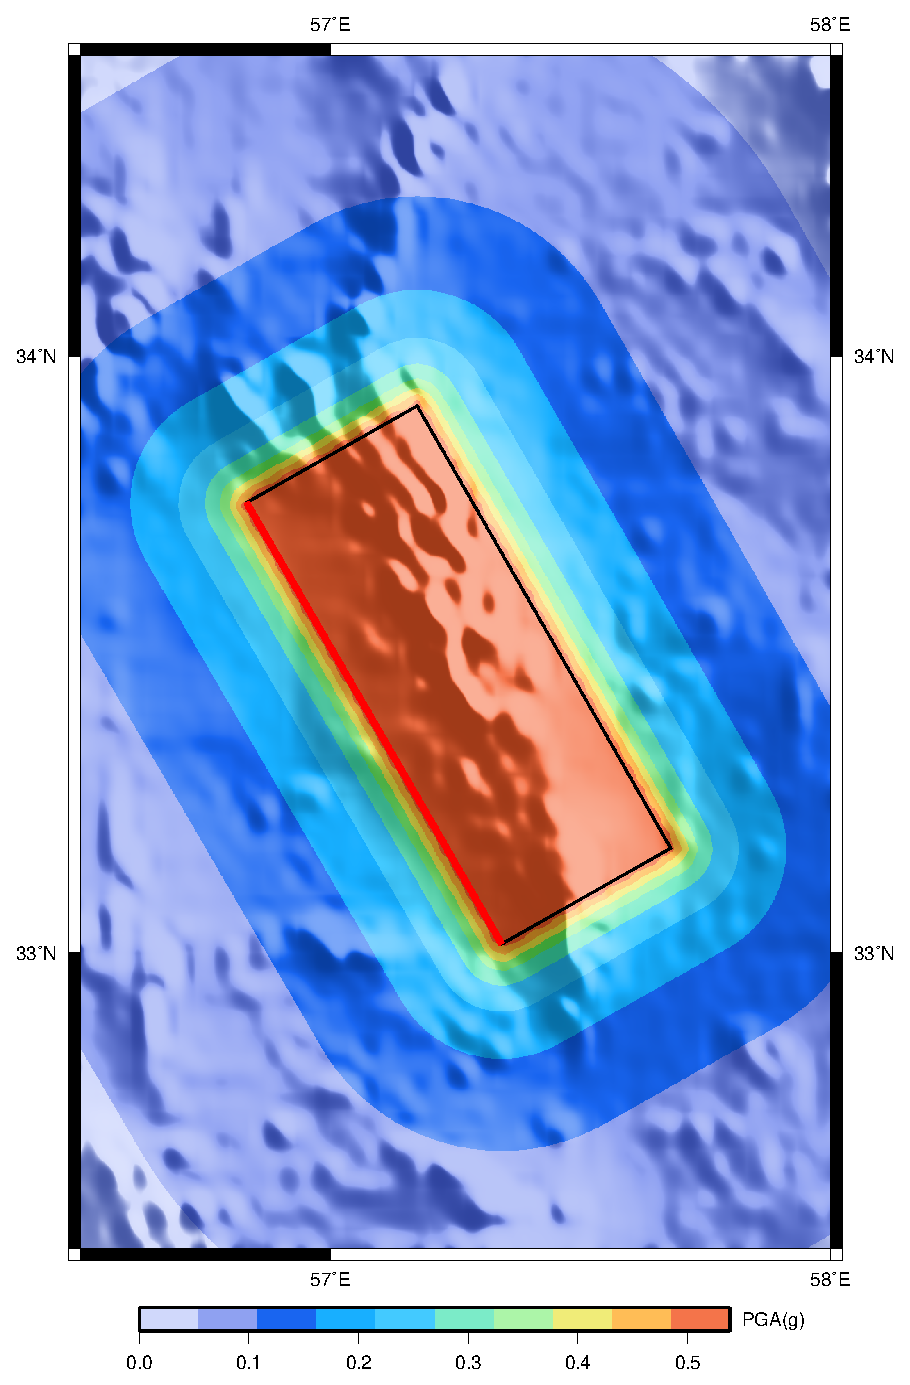
\includegraphics[width=5cm]{./Figures/Part_Hazard/medianGmfTabasPGA.eps}}
\subfigure[]{
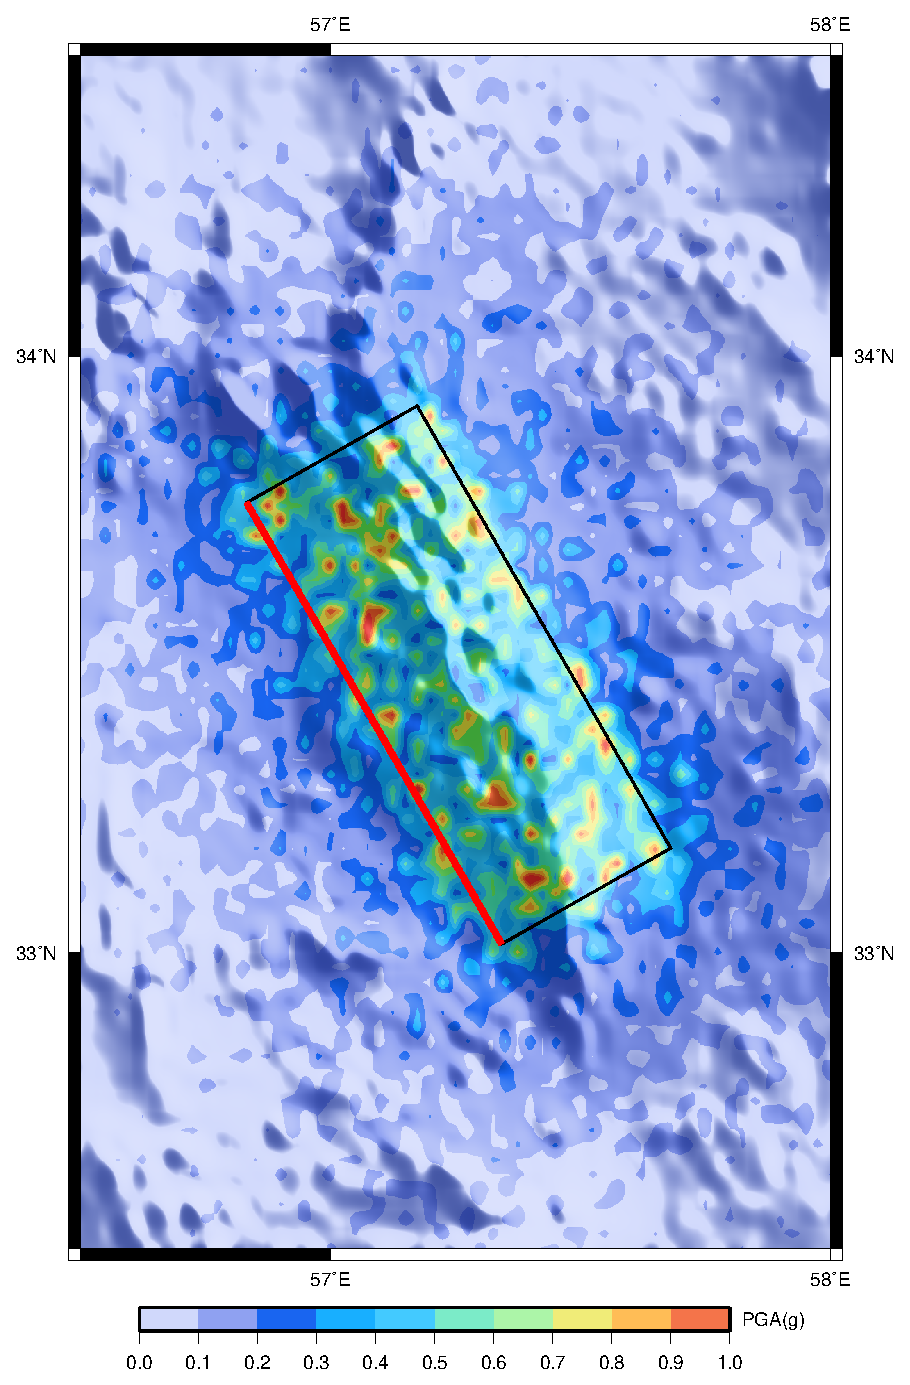
\includegraphics[width=5cm]{./Figures/Part_Hazard/uncorrelatedGmfTabasPGA.eps}}
\subfigure[]{
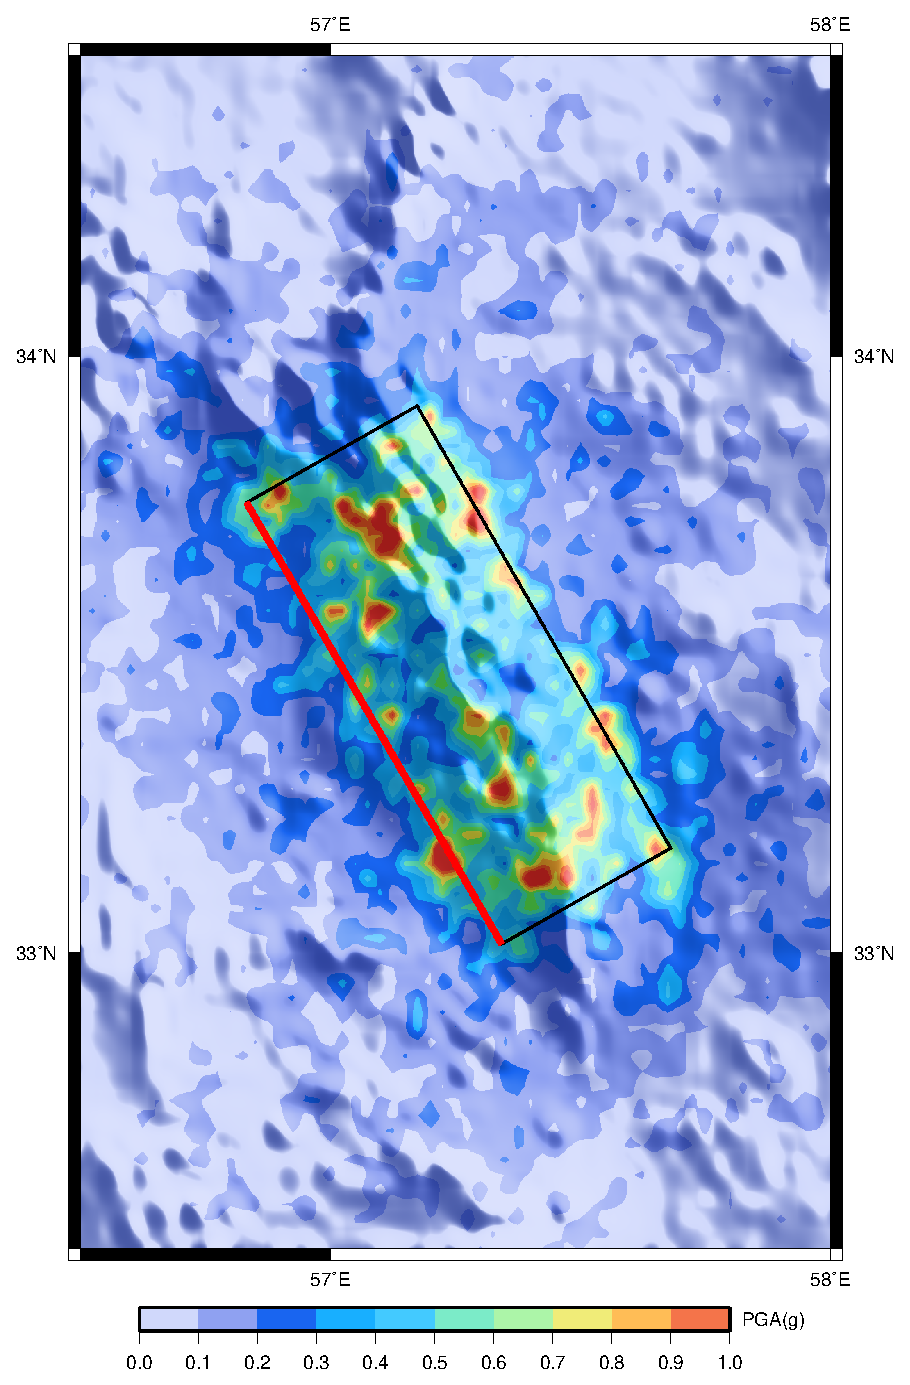
\includegraphics[width=5cm]{./Figures/Part_Hazard/correlatedGmfTabasPGA.eps}}
\subfigure[]{
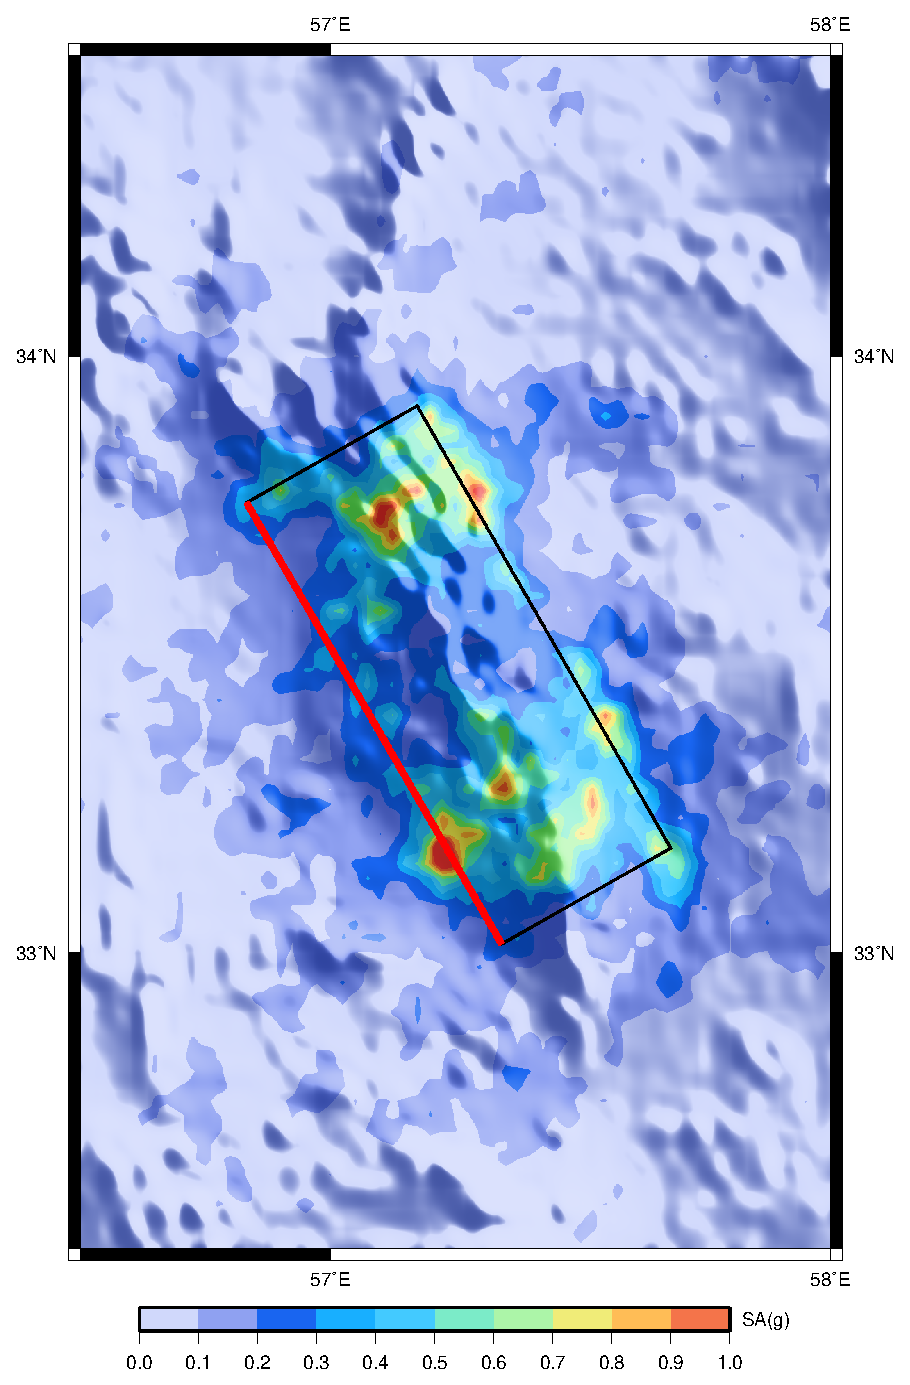
\includegraphics[width=5cm]{./Figures/Part_Hazard/correlatedGmfTabasSA.eps}}
\caption{Examples of median (a), intra-event uncorrelated (b), intra-event 
correlated for PGA (c) and for SA at $T=1$s (d). A rectangular planar rupture 
is considered as source of the shaking (the red line depicts the rupture trace,
and the black line the rupture border). The rupture is associated to a 
magnitude 7 earthquake. The ground motion is estimated using the 
\citet{boore2008} ground motion prediction equation.}
\label{fig:gmfs}
\end{figure}
